\section{Auswertung}
\label{sec:Auswertung}
Alle Berechnungen werden mit dem Programm \glqq Numpy" \cite{numpy}, die Unsicherheiten mit dem Modul \glqq Uncertainties" \cite{uncertainties}, die Ausgleichsrechnungen mit dem Modul \glqq Scipy" \cite{scipy} durchgeführt und die grafischen Darstellungen über das Modul \glqq Matplotlib" \cite{matplotlib} erstellt.


\subsection{Bestimmung des Magnetfeldes}

Mit einer Hallsonde wird das Magnetfeld $B$ abhängig vom angelegten Strom $I$ gemessen, wobei der Strom schrittweise variiert wird. Die Messdaten
sind in Tabelle \ref{tab:mag_verlauf} zu sehen. Der Verlauf der magnetischen Flussdichte in Abhängigkeit der Stromstärke ist zusammen mit einer Ausgleichskurve 
in Plot \ref{fig:mag_verlauf} zu sehen. Die Funktion der Ausgleichskurve ist dabei 
\begin{equation}
     f(x) = ax^3 + bx^2 + cx + d\,.
\end{equation}


\begin{table}
    \centering
    \caption{Messwerte der Magnetfeldstärke}
    \label{tab:mag_verlauf}
    \sisetup{table-format = 1.2}
    \begin{tabular}{S S }
        \toprule
        $I / \si{\ampere}$ & $B / \si{\milli\tesla}$\\
        \midrule
        5.0 & 438.6 \\
        4.5 & 406.5 \\
        4.0 & 370.5 \\
        3.5 & 328.4 \\
        3.0 & 283.2 \\
        2.5 & 240.8 \\
        2.0 & 194.0 \\
        1.5 & 146.4 \\
        1.0 & 99.9 \\
        0.5 & 53.3 \\
        0.0 & 6.5 \\
        \bottomrule
    \end{tabular}
\end{table}

\begin{figure}
    \centering
    \includegraphics[width=\textwidth]{build/b_kurve.pdf}
    \caption{Verlauf des Magnetfeldes in Abhängigkeit der Stromstärke$I$}
    \label{fig:mag_verlauf}
\end{figure}

Damit ergeben sich die Parameter 
\begin{align*}
    a &= \SI{-0.846(118)}{\milli\tesla} \\
    b &= \SI{3.607 (898)}{\milli\tesla} \\
    c &= \SI{89.552(876)}{\milli\tesla} \\
    d &= \SI{7.089 (030)}{\milli\tesla}
\end{align*}

\subsection{Blaue Spektrallinie}

\begin{figure}
    \centering
    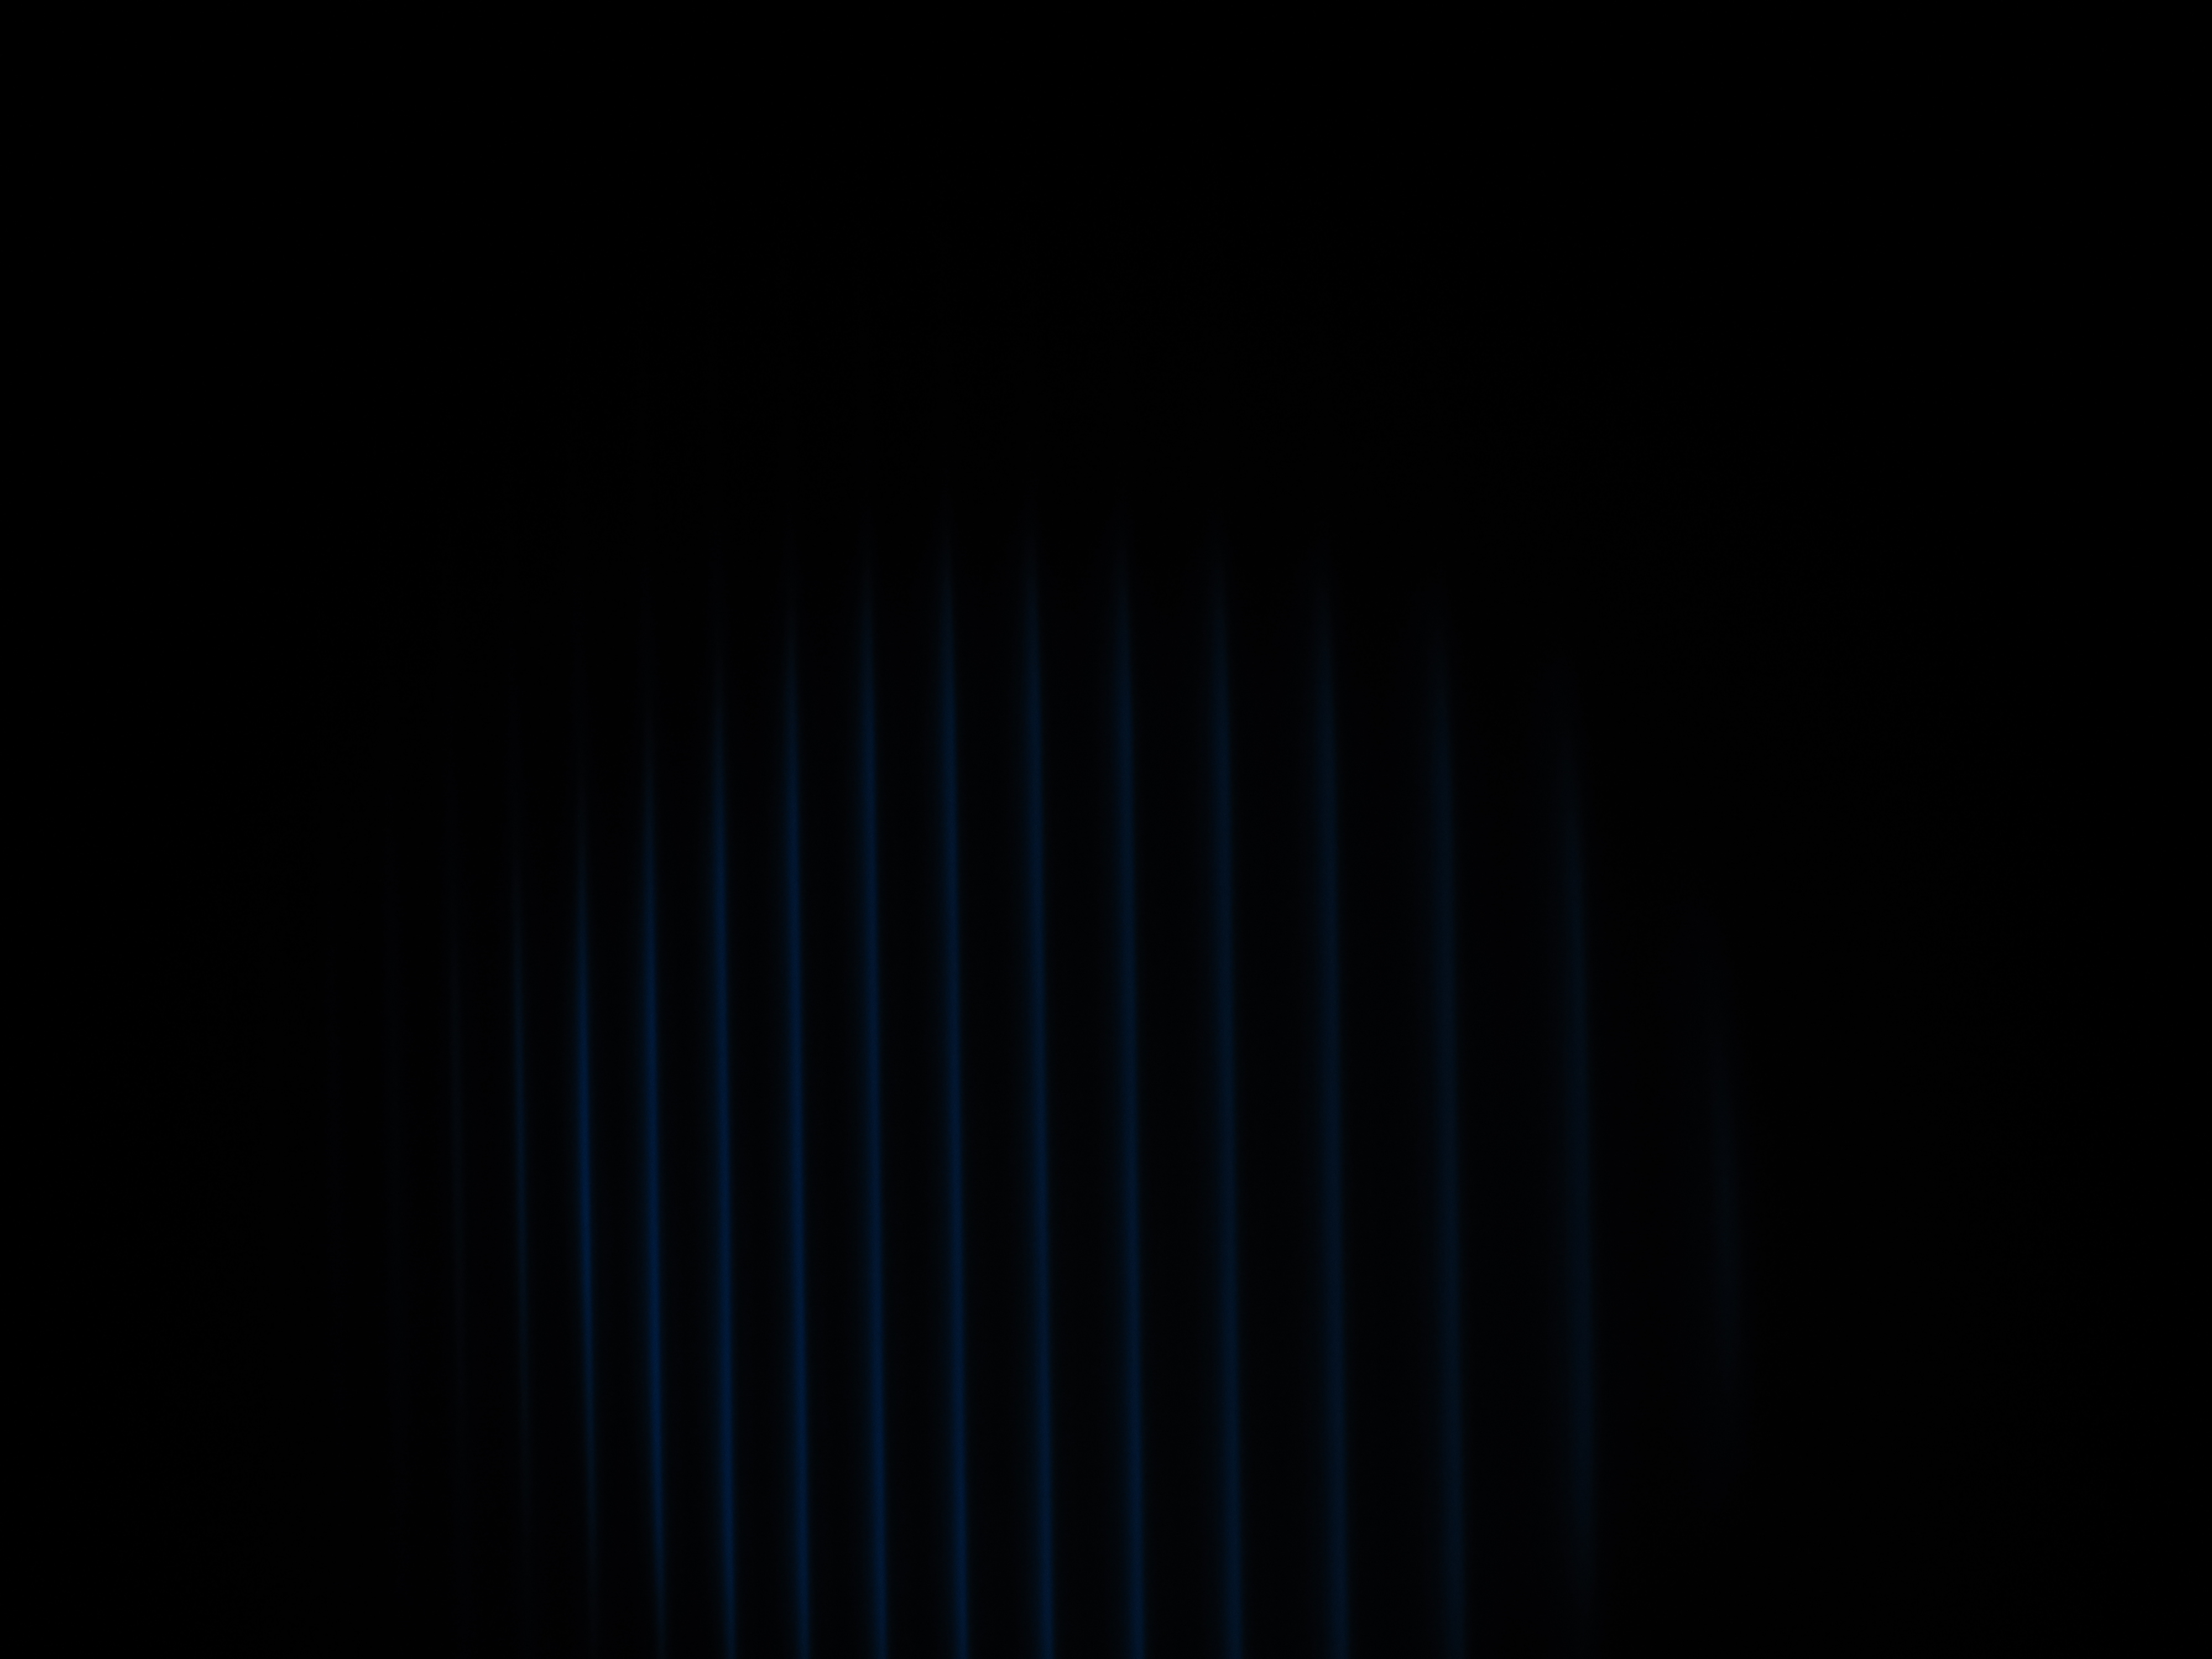
\includegraphics[width=\textwidth]{fotos/blau_0.JPG}
    \caption{Blaue Spektrallinie ohne Magnetfeld.}
    \label{fig:blau_0}
\end{figure}
\hfill
\begin{figure}
    \centering
    
\includegraphics[width=\textwidth]{fotos/blau_pi.JPG}
    \caption{$\pi$-polarisierte blaue Spektrallinie.}
    \label{fig:blau_pi}
\end{figure}
\FloatBarrier

In den Abbildungen \ref{fig:blau_0} und \ref{fig:blau_pi} sind zwei blaue Spektrallinien übereinander gezeigt. Der obere Teil zeigt die Spektrallinien des blauen Lichts mit 
$\SI{480}{\nano\metre}$ Wellenlänge im ungestörten Zustand. Der untere Teil zeigt die Spektrallinien des $\pi$-polarisierten Lichts bei 
angelegtem Magnetfeld. Zur Vermessung der Bilder wird Paint verwendet, um die Abstände der Maxima zueinander in der Einheit Pixel zu messen. 
Dabei ist $\Delta s$ der Abstand zwischen den Maxima im ungestörten Zustand und $\delta s$ dieser Abstand beim $\pi$-polarisierten Licht. 
Aus diesen Werten lassen sich dann anhand der Gleichung 

\begin{equation}
    \delta\lambda = \frac{1}2 \frac{\delta s}{\Delta s} \Delta\lambda_D
\end{equation}

die Wellenlängenverschiebung bestimmen, wobei für die blaue Spektrallinie $\Delta\lambda_D = \SI{26.5}{\pico\metre}$ ist. Da die Abstände in Pixeln in diesem Fall per Hand abgelesen 
wurden, wird beim Fehler von $\delta\lambda$ mit einer Messunsicherheit von 4 Pixeln gerechnet. \\

\begin{table}
    \centering
    \caption{ Abstände der Maxima bei blauer Spektrallinie ohne Magnetfeld und $\pi-$polarisiert. }
    \label{tab:maxima_blau_pi}
    %\sisetup{table-format = 1.2}
    \begin{tabular}{S S S S}
        \toprule
        $\text{Ordnung}$ & $\Delta s \, /\text{Pixel}$  & $\delta s \, /\text{Pixel}$ & $\delta\lambda \, / \, \si{\nano\meter}$  \\
        \midrule
        1  & 116(4) & 25(4)  & 2.904(476) \\
        2  & 122(4) & 25(4)  & 2.761(450) \\
        3  & 129(4) & 26(4)  & 2.715(426) \\
        4  & 134(4) & 27(4)  & 2.715(410) \\
        5  & 139(4) & 27(4)  & 2.617(395) \\
        6  & 146(4) & 28(4)  & 2.584(375) \\
        7  & 154(4) & 35(4)  & 3.063(358) \\
        8  & 163(4) & 34(4)  & 2.810(337) \\
        9  & 175(4) & 36(4)  & 2.772(315) \\
        10 & 191(4) & 40(4)  & 2.822(289) \\
        11 & 208(4) & 42(4)  & 2.721(264) \\                   
        \bottomrule

    \end{tabular}
\end{table}

Aus den Messwerten, wie sie in Tabelle \ref{tab:maxima_blau_pi} aufgeführt sind, kann dann ein Mittelwert für $\delta\lambda_{\pi,\text{blau}}$ gebildet werden. 
Dieser ergibt sich zu 
\begin{equation}
    \delta\lambda_{\pi,\text{blau}} = \SI{2.77(11)}{\pico\m}
\end{equation}

Desweiteren wird für die blaue Spektrallinie der $\sigma-$Übergang untersucht. Hierfür ist das Vorgehen prinzipiell Dasselbe. Es werden wieder 
die gleichen Abstände der Maxima gemessen, nur diesmal wird das $\sigma$-polarisierte Licht betrachtet. Die beiden Spektrallinien werden wieder 
zum Vergleich übereinander gelegt, wie in Abbildung \ref{fig:blau_sigma} zu sehen ist. Die Messdaten zusammen mit den errechneten $\delta\lambda_{\sigma,\text{blau}}$
sind analog zur Vorherigen in der Tabelle \ref{tab:maxima_blau_sigma} dargestellt.\\

\begin{figure}
    \centering
    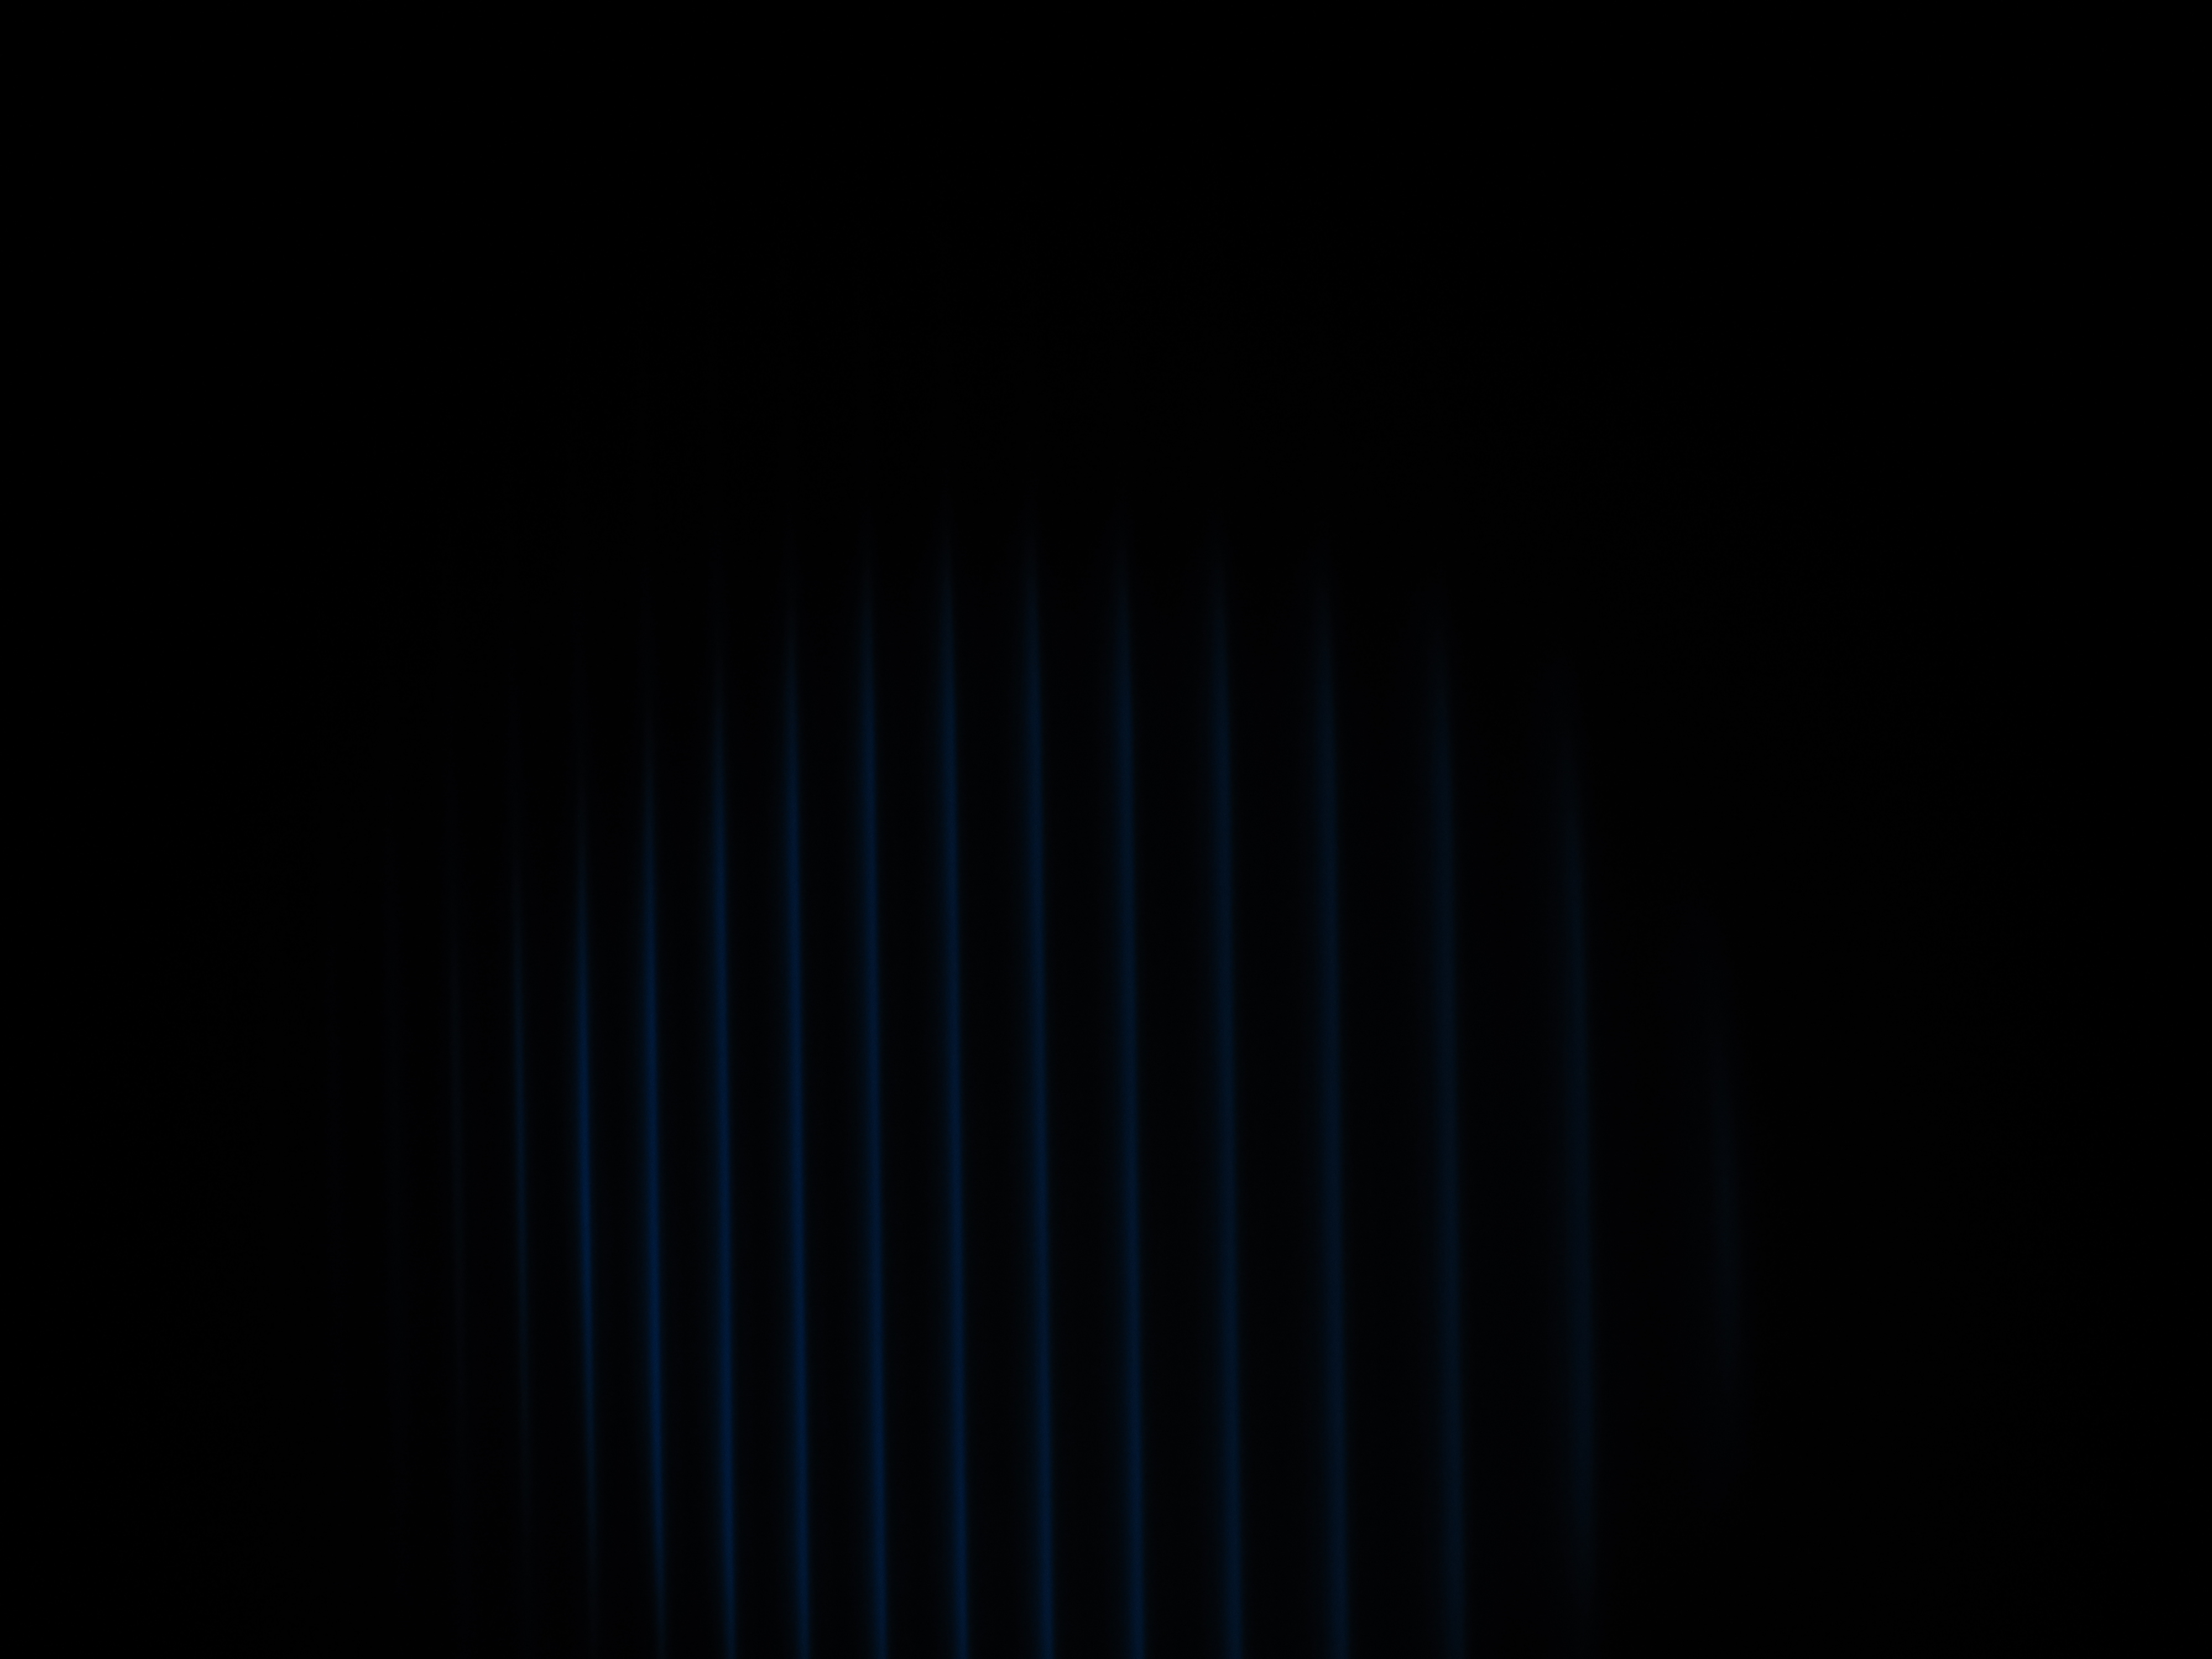
\includegraphics[width=\textwidth]{fotos/blau_0.JPG}
    \caption{Blaue Spektrallinie ohne Magnetfeld.}
    \label{fig:blau_0}
\end{figure}
\hfill
\begin{figure}
    \centering
    
\includegraphics[width=\textwidth]{fotos/blau_sigma.JPG}
    \caption{$\sigma$-polarisierte blaue Spektrallinie.}
    \label{fig:blau_sigma}
\end{figure}
\FloatBarrier

\begin{table}
    \centering
    \caption{Abstände der Maxima bei blauer Spektrallinie ohne Magnetfeld und $\sigma-$polarisiert.}
    \label{tab:maxima_blau_sigma}
    \sisetup{table-format = 1.2}
    \begin{tabular}{S S S S}
        \toprule
        $\text{Ordnung}$ & $\Delta s \, /\text{Pixel}$  & $\delta s \, /\text{Pixel}$ & $\delta\lambda \, / \, \si{\nano\meter}$  \\
        \midrule
        1  & 116(4)  & 52(4) & 6.041(509) \\
        2  & 122(4)  & 59(4) & 6.516(491) \\
        3  & 129(4)  & 57(4) & 5.954(456) \\
        4  & 134(4)  & 61(4) & 6.134(441) \\
        5  & 139(4)  & 64(4) & 6.204(426) \\
        6  & 146(4)  & 66(4) & 6.091(405) \\ 
        7  & 154(4)  & 69(4) & 6.037(383) \\
        8  & 163(4)  & 76(4) & 6.282(364) \\ 
        9  & 175(4)  & 84(4) & 6.468(342) \\
        10 & 191(4)  & 86(4) & 6.067(309) \\
        11 & 208(4)  & 97(4) & 6.284(285) \\
        \bottomrule

    \end{tabular}
\end{table}

Daraus lässt sich dann der Mittelwert von $\delta\lambda_{\sigma,\text{blau}}$ zu 
\begin{equation}
    \delta\lambda_{\sigma,\text{blau}} = \SI{6.19(12)}{\pico\m}
\end{equation}
bestimmen. 

\subsection{Rote Spektrallinie}

\begin{figure}
    \centering
    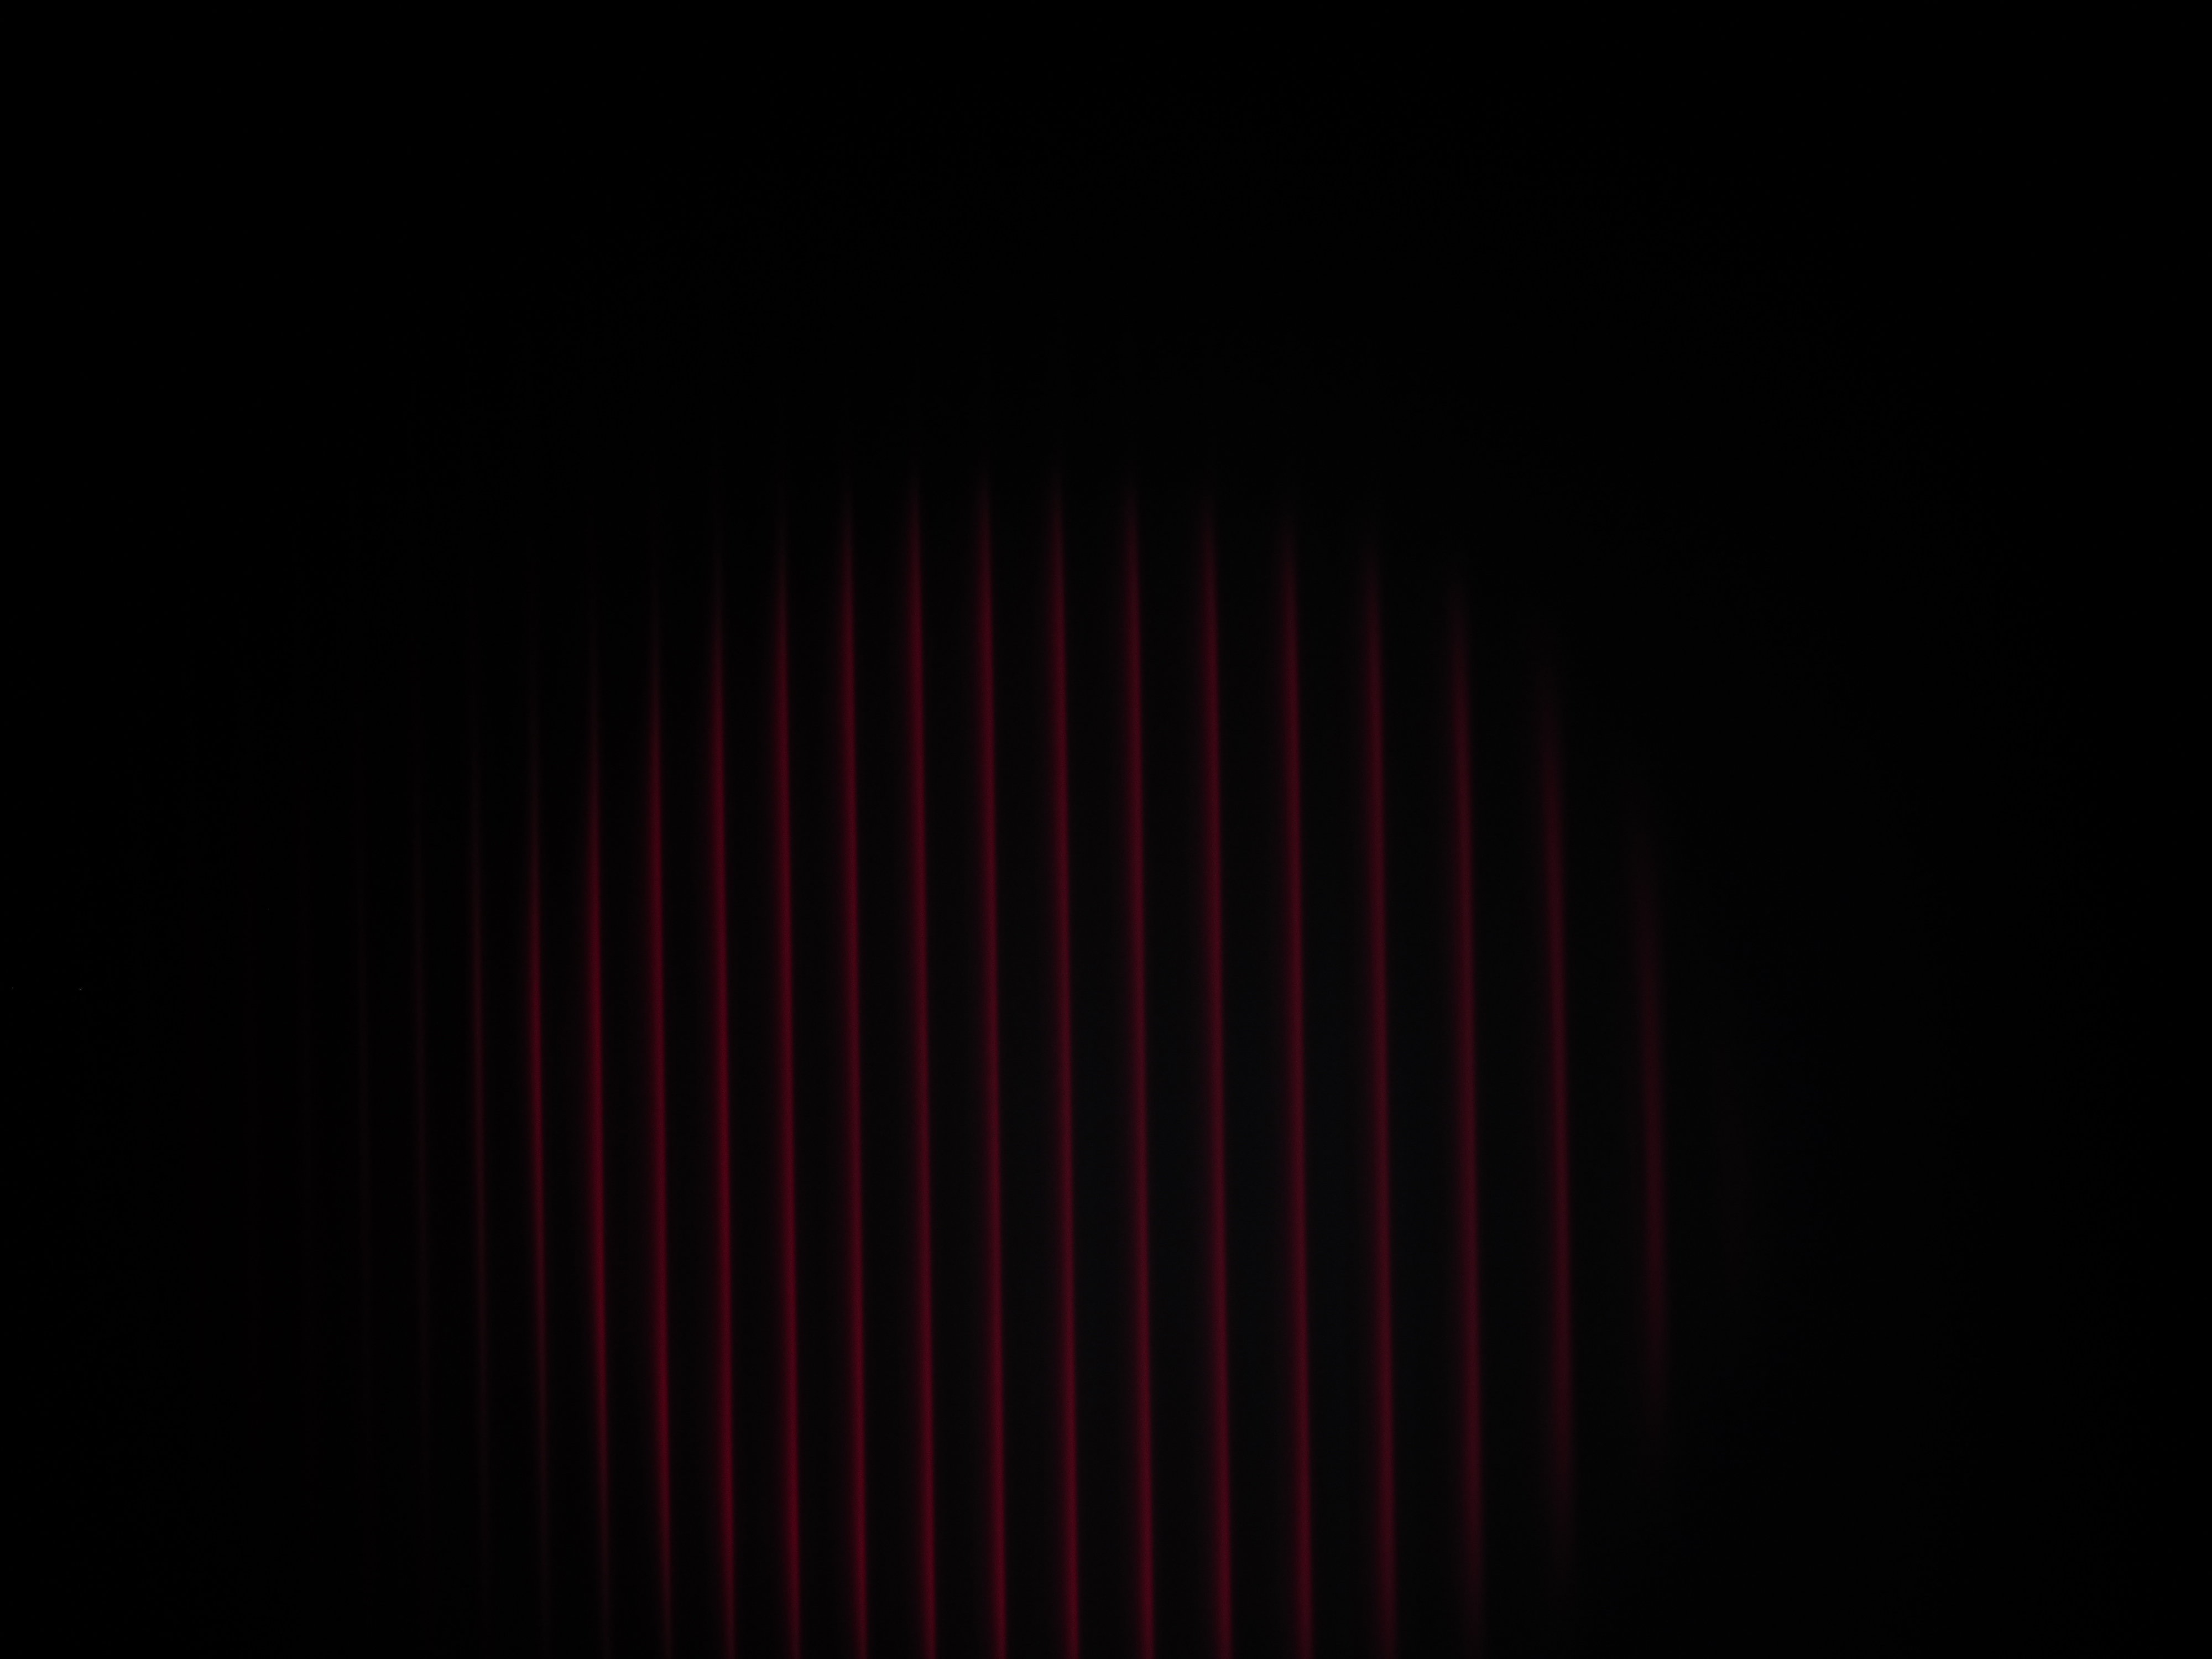
\includegraphics[width=\textwidth]{fotos/rot_0.JPG}
    \caption{Rote Spektrallinie ohne Magnetfeld.}
    \label{fig:rot_0}
\end{figure}
\hfill
\begin{figure}
    \centering
    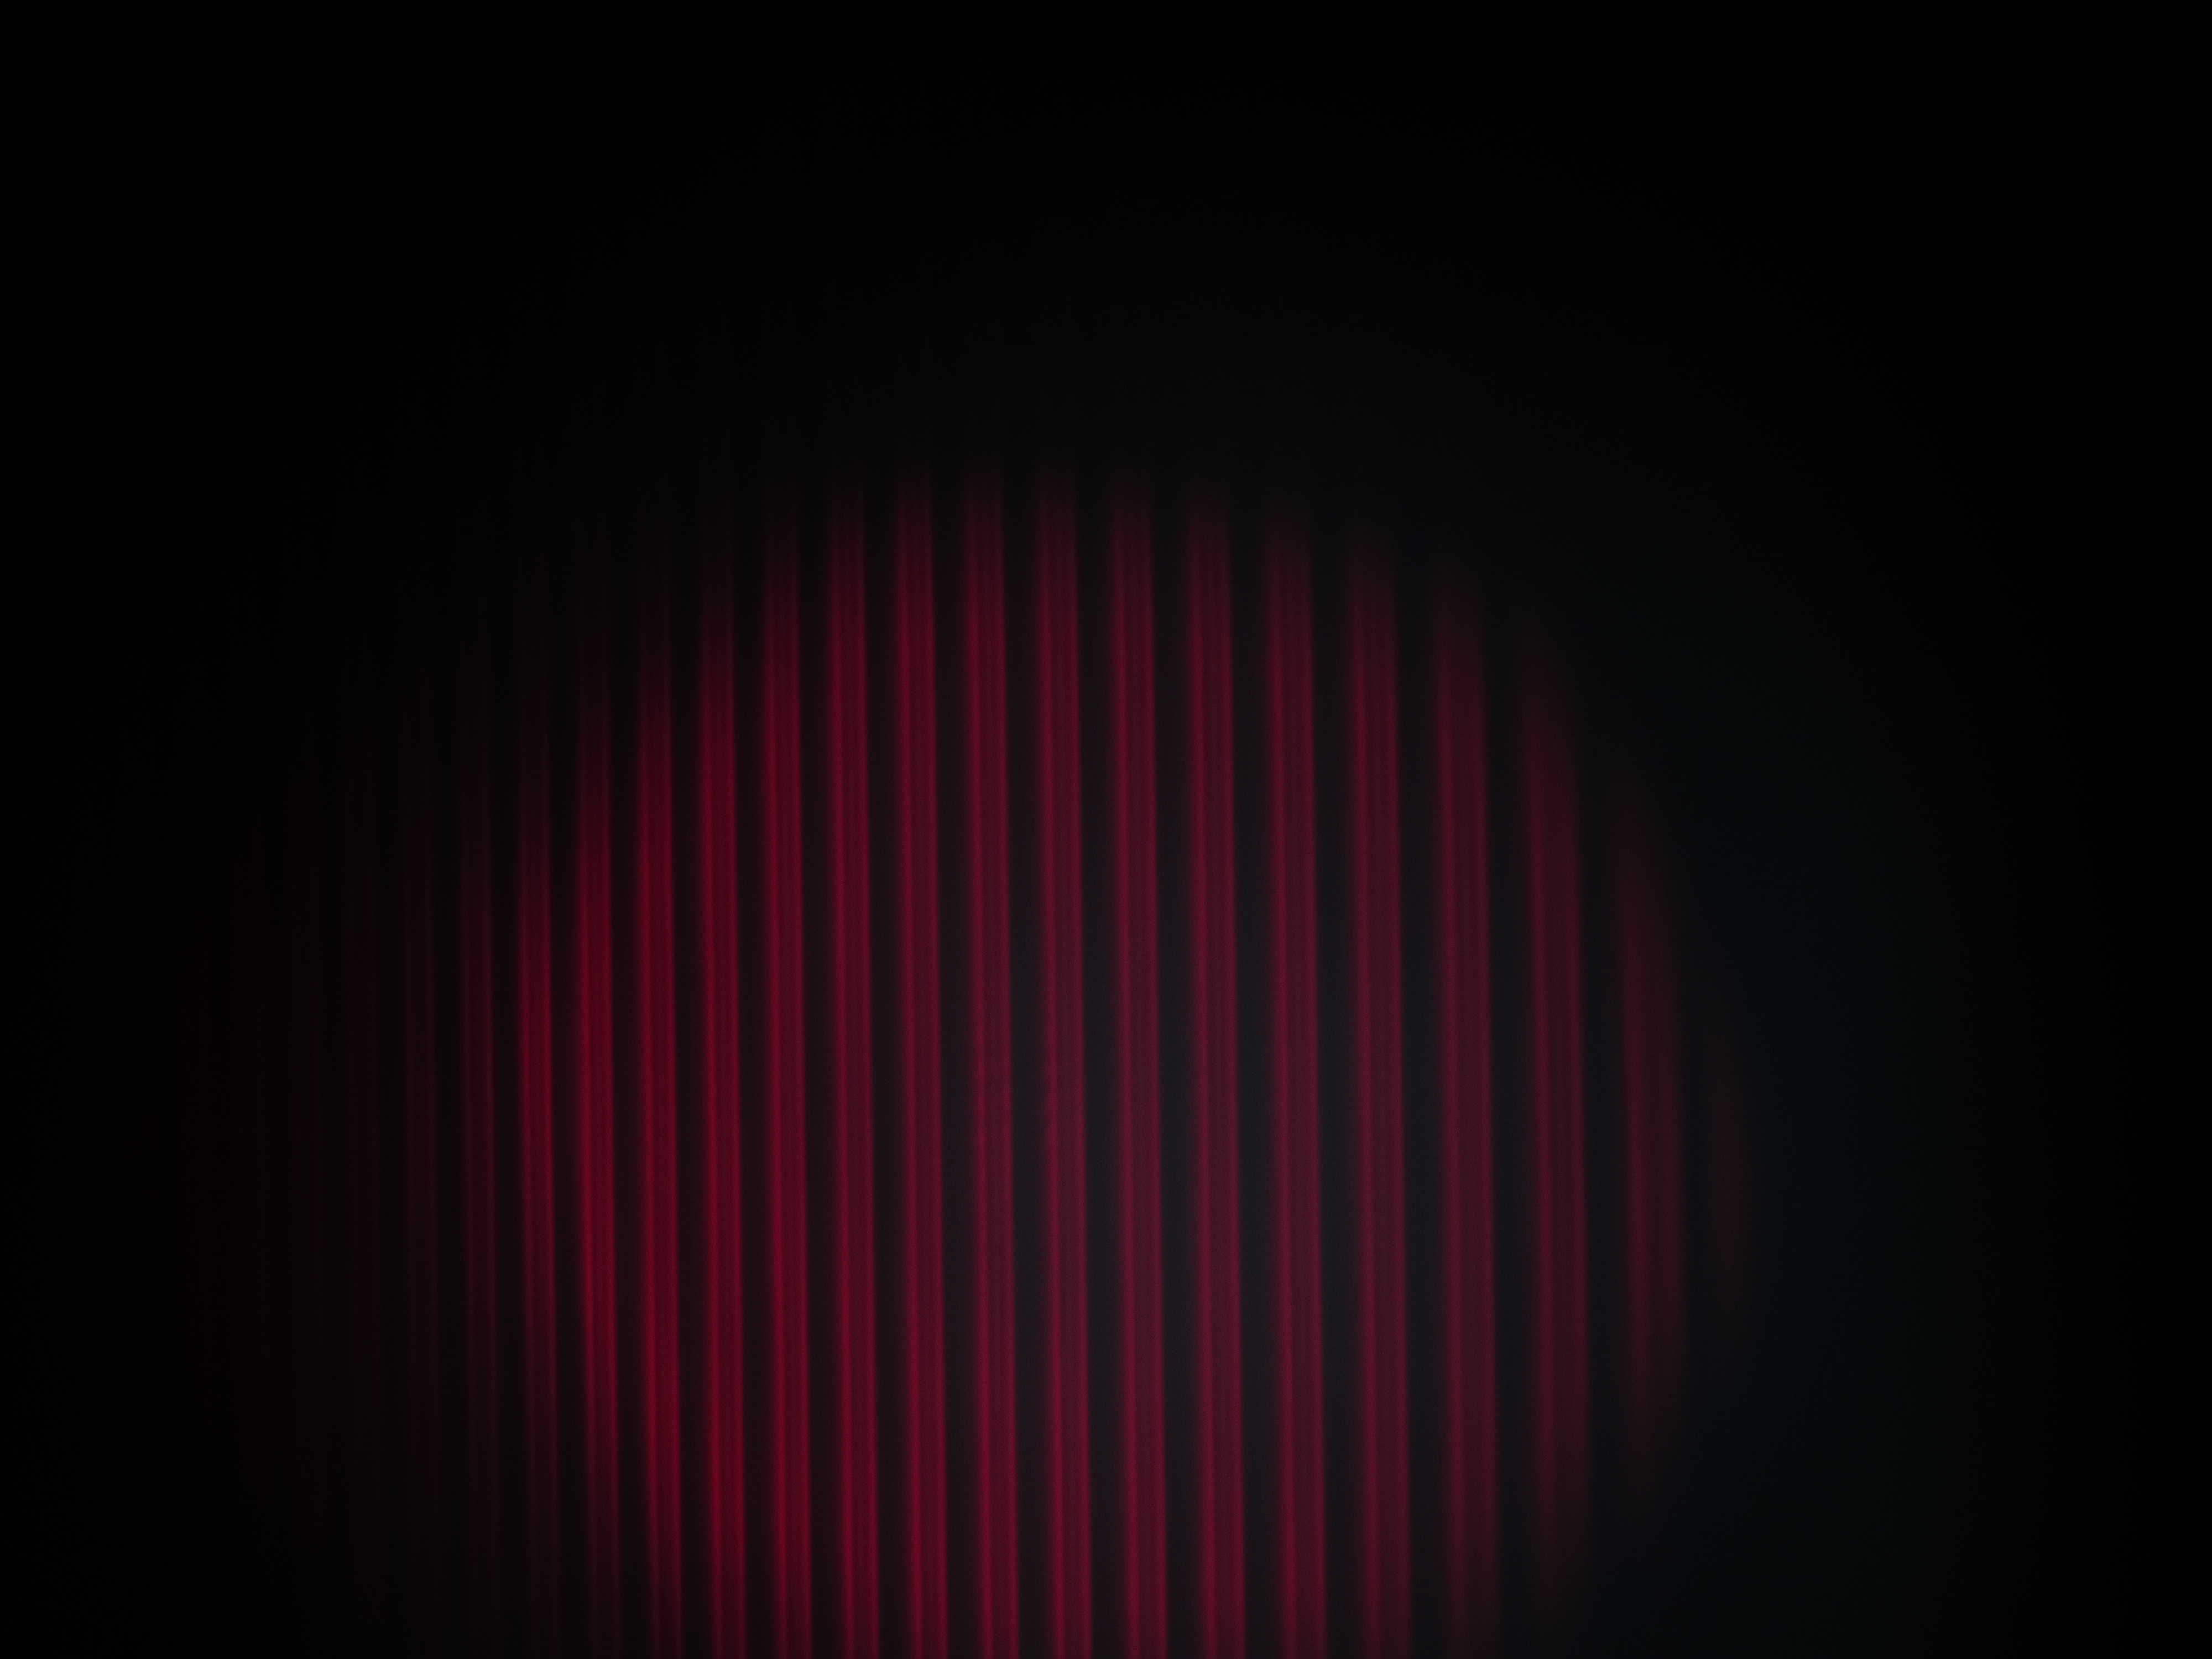
\includegraphics[width=\textwidth]{fotos/rot_sigma.JPG}
    \caption{$\sigma$-polarisierte rote Spektrallinie.}
    \label{fig:rot_sigma}
\end{figure}
\FloatBarrier
Für die rote Spektrallinie wird ebenfalls die $\sigma-$Linie untersucht, indem das gleiche Verfahren, wie für die blaue Spektrallinie 
angewendet wird. Abbildung \ref{fig:rot_sigma} zeigt Hierfür ebenfalls die beiden Spektrallinien, ungestört und im Magnetfeld, übereinander. In der Tabelle \ref{tab:maxima_rot_sigma}
sind auch wieder analog die Messdaten aufgeführt.\\

\begin{table}
    \centering
    \caption{Abstände der Maxima bei roter Spektrallinie ohne Magnetfeld und $\sigma-$polarisiert.}
    \label{tab:maxima_rot_sigma}
    \sisetup{table-format = 1.2}
    \begin{tabular}{S S S S}
        \toprule
        $\text{Ordnung}$ & $\Delta s \, /\text{Pixel}$  & $\delta s \, /\text{Pixel}$ & $\delta\lambda \, / \, \si{\nano\meter}$  \\
        \midrule
        1  & 114(4) & 40(4)  &  8.578(909) \\ 
        2  & 114(4) & 42(4)  &  9.007(914) \\
        3  & 117(4) & 42(4)  &  8.776(888) \\
        4  & 122(4) & 41(4)  &  8.216(845) \\
        5  & 122(4) & 44(4)  &  8.818(852) \\ 
        6  & 128(4) & 45(4)  &  8.595(809) \\
        7  & 130(4) & 44(4)  &  8.275(794) \\
        8  & 135(4) & 47(4)  &  8.512(767) \\
        9  & 140(4) & 48(4)  &  8.382(738) \\
        10 & 145(4) & 49(4)  &  8.262(711) \\
        11 & 151(4) & 49(4)  &  7.934(680) \\
        \bottomrule

    \end{tabular}
\end{table}

Aus diesen ergibt sich für den Mittelwert von $\delta\lambda_{\sigma,\text{rot}}$
\begin{equation}
    \delta\lambda_{\sigma,\text{rot}} = \SI{8.49(25)}{\pico\m}
\end{equation}

\subsection{Landé-Faktoren}

Die Berechnung der Landé-Faktoren erfolgt über die Gleichung \ref{eqn:lande}. Die Aus den Messdaten berechneten Landé-Faktoren  
sind in der Tabelle \ref{tab:lande} dargestellt. Der Fehler für den Landé-Faktor lässt sich dabei über 
\begin{equation}
    F(g) = \frac{hc}{\lambda^2 \mu _\text{B}} \sqrt{\left ( \frac{1}{B} F(\delta \lambda) \right)^2}
\end{equation} bestimmen. 

\begin{table}
    \centering
    \caption{Landé-Faktoren}
    \label{tab:lande}
    \sisetup{table-format = 1.2}
    \begin{tabular}{S S S S}
        \toprule
        {$\lambda / \si{\nano\meter}$} & {$\text{Polarisierung}$ }& {$B / \si{\milli\tesla}$} & {$\text{Landé-Faktor}$} \\
        \midrule
        480   &  {$\pi$}    & \num{0.441(029)} & \num{0.58(05)} \\
        480   &  $\sigma$ &   \num{0.314(013)} & \num{1.83(08)} \\   
        644   &  $\sigma$ &   \num{0.441(029)} & \num{0.99(07)} \\         
        \bottomrule

    \end{tabular}
\end{table}
